\chapter{Oscillators}
Usually, what we want to do when applying feedback is to control the loop gain $T(j\omega)$ such that the amplifier becomes and stays stable. However, in this chapter we try to do the opposite: for a certain frequency $\omega_0$, we design the circuit such that $T(j\omega_0) = H(j\omega_0) A(j\omega_0) = 1$. Note how this is different from the condition in chapter \ref{ch:feedback}: we assume here that the feedback signal is \emph{added} to the input signal.\\
This means that the circuit will be unstable for one single frequency $\omega_0$. These circuits generate sinusoidal output signals at $\omega_0$, even when there is no signal at the input\footnote{There is always \emph{noise} present, and white noise contains every frequency. This will be studied in other courses}. We call them \emph{oscillators}.

\section{Phase Shift Oscillator}
This oscillator consists of a single common-emitter amplifier that (a) provides the gain and (b) provides a 180° phase shift. To generate the other 180° phase shift, $3$ RC blocks are placed in series at the output of the amplifier, as in figure \ref{fig:phaseshift1}. So we have an amplifier, followed by feedback loop of 3 RC blocks, that couple the output signal back to the input.  If each $RC$ circuit could function independent from the others, we could just tune $R$ and $C$ to provide a $60$° shift for a required frequency $\omega_0$. However, because each next block loads the previous one, the calculation is more complicated.\\
\begin{figure}[h!]
	\centering
	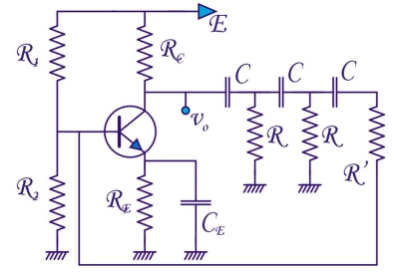
\includegraphics[width=8cm]{figures/ch11/phaseshift1.jpg}
	\caption{}
	\label{fig:phaseshift1}
\end{figure}
To determine $\omega_0$, we establish the AC equivalent circuit as in figure \ref{fig:phaseshift2}  - with $R_{eq} = r_c || R_C$ and $R_\pi = r_\pi || R_1 || R_2$ - and compute the loop gain $T(j\omega)$. Then we verify the oscillation conditions:
\begin{itemize}
	\item $|T(j\omega_0)| = 1$
	\item $\angle T(j\omega_0) = 0$
\end{itemize}
so for one frequency, the signal travels around the loop and arrives in phase and with the same magnitude back at the input\footnote{If $|T(j\omega_0)| > 1$, we wont get a nice sinusoid but a block signal at the output.} This condition also implies that $\Im m\{T(j\omega)\} = 0$ and $\Re e\{T(j\omega)\} = 1$.\\
To compute the loop gain, we cut the link between the input and output of the transistor, and compute which $v_{be}'$ at $R_\pi$ will be generated by the current source $g\;v_{be}$. The loop gain is then $T = \frac{v_{be}'}{v_{be}}$. The resistance $R'$ is chosen such that $R_\pi + R'  = R$.\\
From the AC equivalent circuit, we find:
$$
-gv_{be} = -gR_\pi i_b \approx i_b \bigg( 3 + \frac{4}{j\omega RC} - \frac{1}{\omega^2 R^2 C^2} + \frac{R}{R_{eq}} + \frac{6}{j\omega R_{eq} C} - \frac{5}{\omega^2C^2RR_{eq}} - \frac{1}{j\omega^3 R^2 R_{eq} C^3} \bigg)
$$
The imaginary part gives us $\omega_0$:
\begin{align*}
	\frac{4}{RC} + \frac{6}{R_{eq} C} - \frac{1}{\omega_0^2 R^2 R_{eq} C^3} = 0\\
	\Rightarrow \frac{4}{R} + \frac{6}{R_{eq}} = \frac{1}{\omega_0^2 R^2 R_{eq} C^2}\\
	\Rightarrow 4R_{eq} + 6R = \frac{1}{\omega_0^2 R C^2}\\
	\Rightarrow  \omega_0^2 = \frac{1}{(4R_{eq} + 6R) R C^2}\\
\end{align*}


\begin{figure}[h!]
	\centering
	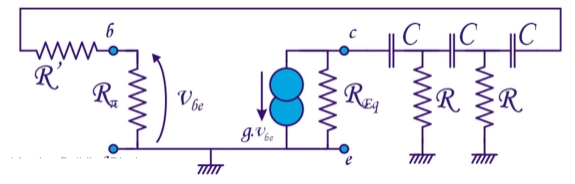
\includegraphics[width=12cm]{figures/ch11/phaseshift2.jpg}
	\caption{}
	\label{fig:phaseshift2}
\end{figure}

The real part provides the criterion for oscillation:
\begin{align*}
	-gR_\pi = 3 + \frac{1}{\omega^2 R^2 C^2} + \frac{R}{R_{eq}} - \frac{5}{\omega^2C^2RR_{eq}} \\
	\Rightarrow -gR_\pi = 3 - \frac{6R + 4R_{eq}}{R} + \frac{R}{R_{eq}} - \frac{5(6R + 4R_{eq})}{R_{eq}}\\
	(gR_\pi - 23) + 4 \frac{R_{eq}}{R} - 29 \frac{R}{R_{eq}} = 0
\end{align*}
This equation can be solved for the ratio $\frac{R}{R_{eq}}$:
$$
\frac{R}{R_{eq}} = \frac{gR_\pi - 23}{58} + \sqrt{\frac{(gR_\pi - 23)^2 - 464}{58}}
$$
This equation only has a solution only if $gR_\pi > 23 + \sqrt{464} \approx 44.6$, which puts a lower limit on the transconductance $g$ and so on the bias current $I_{CQ}$ of the amplifier. If $g$ is is higher, the output will be distorted; if it is lower, there will be no oscillation.
\section{Wien Bridge Oscillator}
\label{sec:wien_bridge}

The Wien bridge oscillator from figure \ref{fig:wienbridge1} is a popular oscillator that uses an OPAMP with two feedback loops:
\begin{itemize}
	\item One stable loop through resistances $R_S$ and $R_F$
	\item An unstable loop (on the positive terminal) through $C$ in series with $R$ (= $Z_F$), and $C$ in parallel with $R$ (= $Z_S$):
	\begin{align*}
		Z_F = R + \frac{1}{j\omega C} = \frac{1+ j RC \omega}{j\omega C} \\
		Z_S = R || \frac{1}{j\omega C} = \frac{R}{1+ j RC \omega}\\
	\end{align*}
\end{itemize}

\begin{figure}[h!]
	\centering
	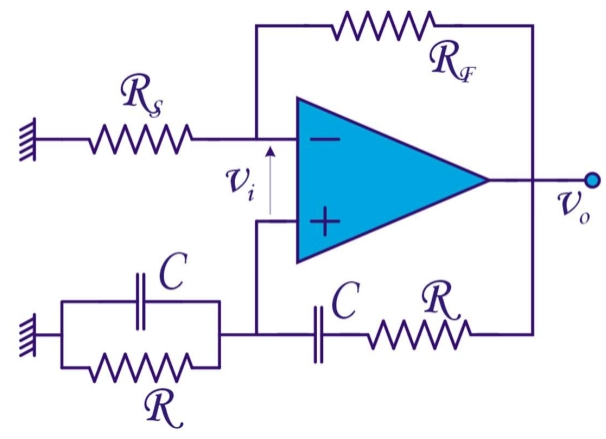
\includegraphics[width=8cm]{figures/ch11/wienbridge1.jpg}
	\caption{}
	\label{fig:wienbridge1}
\end{figure}

The loop gain can be found by computing the input of the OPAMP $v_i = v_p - v_n$ and by setting $v_o = A v_i$. This comes down to cutting the loop at the output of the amplifier, injecting a signal $v_t$ into the feedback path and computing $v_o$:
\begin{align*}
	v_n &= \frac{R_S}{R_S + R_F} v_o\\
	v_p &= \frac{Z_S}{Z_S + Z_F} v_o = \frac{j\omega RC}{1 + j3RC\omega - R^2C^2\omega^2} v_o\\
	v_o &= A\; v_i = A\; (v_p - v_n) \\
				&= A \bigg( \frac{j\omega RC}{1 + j3RC\omega - R^2C^2\omega^2} - \frac{R_S}{R_S + R_F} \bigg) v_o
\end{align*}
With $A \gg 1$, this becomes:
\begin{align*}
	\frac{j\omega RC}{1 + j3RC\omega - R^2C^2\omega^2} \approx \frac{R_S}{R_S + R_F} = k \\
	\Rightarrow j\omega RC = k + j\omega 3kRC - \omega^2 k R^2 C^2
\end{align*}
In this case, the real part gives $\omega_0$:
\begin{align*}
	k - \omega_0^2 k R^2 C^2 = 0 \\
	\Rightarrow \omega_0 = \frac{1}{RC}
\end{align*}
and the oscillation condition is given by the imaginary part:
\begin{align*}
	j\omega RC = j\omega 3kRC \\
	\Rightarrow k = \frac{R_S}{R_S + R_F} = \frac{1}{3}
\end{align*}


\section{Colpitts Oscillator}
\label{sec:colpitts}

A Colpitts oscillator is an oscillator that's very popular in radio application. It consists of a common-emitter amplifier followed by an inductor and two capacitors in the feedback path. 

\begin{figure}[h!]
	\centering
	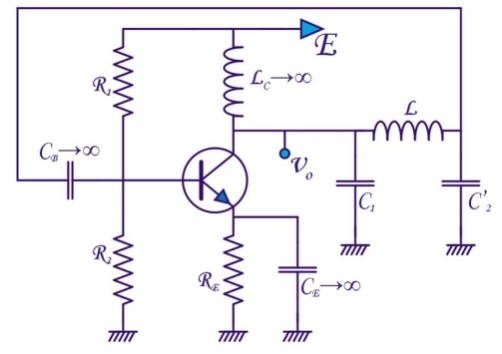
\includegraphics[width=8cm]{figures/ch11/collpits1.jpg}
	\caption{}
	\label{fig:collpits1}
\end{figure}

Inductor $L_C$ and capacitor $C_B$ are used for respectively biasing and coupling in the signal, as seen previously. The same goes for capacitor $C_E$, which short-circuits $R_E$. We can thus omit them from the AC equivalent circuit in figure \ref{fig:collpits2}, where we do consider the parasitic transistor capacitances $c_\pi$ and $c_\mu$ and replace the latter by the Miller capacitance $C_M$ (i.e. we suppose that the Miller conditions are satisfied).

\begin{minipage}{.7\textwidth}
	\centering
	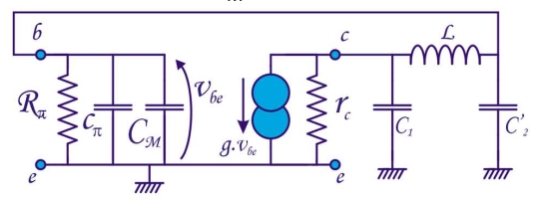
\includegraphics[width=10cm]{figures/ch11/collpits2.jpg}
	\captionof{figure}{}
	\label{fig:collpits2}
\end{minipage}
\begin{minipage}{.3\textwidth}
	\centering
	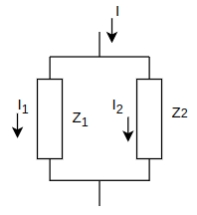
\includegraphics[width=3cm]{figures/ch11/collpits3.jpg}
	\captionof{figure}{}
	\label{fig:collpits3}
\end{minipage}%


We can simplify further by grouping all capacitors between base and ground: $C_2 = c_\pi + C_M + C_2'$. Let $Z_1 = r_c || C_1 = \frac{r_c}{1 + j\omega r_c C_1}$ and $Z_2 = j\omega L + (\frac{1}{j\omega C_2} || R_\pi) = j\omega L + \frac{R_\pi}{1 + j\omega R_\pi C_2}$. As such, $Z_1$ and $Z_2$ are two impedances in parallel and they operate as a current divider (see figure \ref{fig:collpits3}): 
$$
I_2 = \frac{Z_1}{Z_1 + Z_2} I
$$
Like for the phase-shift oscillator, we assume that the base-emitter voltage $v_{be}$ is generated with the current source $-g\;v_{be}$. The current through the parallel combination of $R_\pi$ and $C_2$ is then:
\begin{align*}
	i_{R_\pi||C_2} = -g\;v_{be} \frac{Z_1}{Z_1 + Z2} 
\end{align*}
and $v_{be}$ is equal to:
\begin{align*}
v_{be} &= \frac{R_\pi}{1 + j\omega R_\pi C_2} i_{R_\pi||C_2} = -g\;v_{be} \frac{Z_1}{Z_1 + Z_2} \frac{R_\pi}{1 + j\omega R_\pi C_2} \\
	   &=  -g\;v_{be} \frac{\frac{r_c}{1 + j\omega r_c C_1}}{\frac{r_c}{1 + j\omega r_c C_1} + j\omega L + \frac{R_\pi}{1 + j\omega R_\pi C_2}} \frac{R_\pi}{1 + j\omega R_\pi C_2} \\
	   &= - v_{be} \frac{g r_c R_\pi}{j\omega L (1 + j \omega R_\pi C_2)(1 + j \omega r_c C_1) + R_\pi (1 + j \omega r_c C_1) + r_c (1 + j \omega R_\pi C_2)}
\end{align*}

This last expression results in the condition:
$$
j\omega L -\omega^2 (R_\pi C_2 + r_c C1) L - j\omega^3 r_c R_\pi C_1 C_2 L + R_\pi + j\omega r_c R_\pi C_1 + r_c + j\omega R_\pi r_c C_2 = -g r_c R_\pi
$$
By examining the real parts of this equation, we find $\omega_0$:
\begin{align*}
	\omega_0^2 = \frac{L+ r_c R_\pi (C_1 + C_2)}{r_c R_\pi C_1 C_2 L} = \frac{1}{r_c R_\pi C_1 C_2} + \frac{C_1 + C_2}{C_1 C_2 L} \approx \frac{C_1 + C_2}{C_1 C_2 L} = \frac{1}{C_{eq} L}
\end{align*}
with $C_{eq}$ the parallel combination of $C_1$ and $C_2$. \\
From the imaginary part, the oscillation condition on the transconductance $g$ can be found:
$$
g + \frac{R_\pi + r_c}{r_c R_\pi} \approx \frac{C_1 + C_2}{C_1 C_2 L}(R_\pi C_2 + r_c C_1) 
$$
%\section{Hartley \& Miller Oscillator}

\section{Quartz Oscillator}
Regular oscillators are not very good time references: they drift and have a precision of only $\sim 1\%$. This means that daily they have an error of about $15$ minutes. A \emph{quartz oscillator} - i.e. an oscillator based on the vibrations of quartz crystal - has a much higher precision: from $\sim 10^{-6}$ (1 ppm - about 30 seconds per year) to $\sim 10^{-7}$ if they are kept at a stabilized temperature.\\
Quartz is a mineral composed of silicon and oxygen atoms arranged in a specific crystal structure.  It exhibits a \emph{piezoelectric effect}, which means that it can generate an electric charge when subjected to mechanical stress, such as pressure or vibration. This effect also works in the other way: quartz changes shape when a voltage is applied.

\begin{figure}[h!]
	\centering
	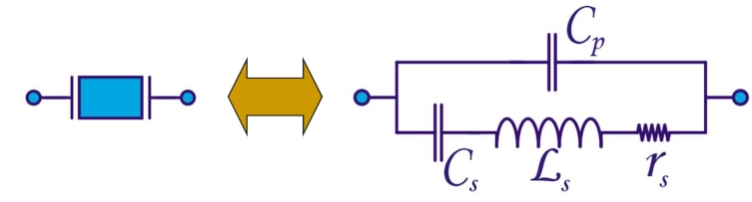
\includegraphics[width=10cm]{figures/ch11/quartz1.jpg}
	\caption{}
	\label{fig:quartz1}
\end{figure}

The quartz crystal with the external clamps is represented by the symbol in the left part of figure \ref{fig:quartz1}. From an electrical point of view, a quartz crystal can be modeled as in the circuit on the right part of the figure. The different components are justified because the moving crystal has several mechanical characteristics for which we use an electrical equivalent:
\begin{itemize}
	\item Stiffness, because you have to provide energy before anything moves: modeled by a capacitor $C_s \sim 10$ fF
	\item Mass, because there is inertia when you have to displace mass: modeled by an inductor $L_s \sim 1000$ H
	\item Friction, because heat is generated when the crystal moves: modeled by a resistance $r_s \sim 100 \; \Omega$
	\item The clamps (due to the external connectors): modeled by a a capacitor $C_p \sim 10$ pF
\end{itemize}
If we ignore $r_s$, we can compute the admittance $Y(j\omega)$ of the quartz crystal:
\begin{align*}
	Y(j\omega) &= j\omega C_p + \frac{1}{j\omega L_s + \frac{1}{j\omega C_s}} = j\omega C_p + \frac{j\omega C_s}{1 - \frac{\omega^2}{\omega_s^2}} \\
			   &= j\omega C_p \frac{\big(1 + \frac{C_s}{C_p} \big) \omega_s^2 - \omega^2}{\omega_s^2 - \omega^2} = j\omega C_p \frac{\omega_p^2 - \omega^2}{\omega_s^2 - \omega^2}
\end{align*}
with important frequencies $\omega_s^2 = \frac{1}{L_s C_s}$ and $\omega_p^2 =  \big(1 + \frac{C_s}{C_p} \big) \omega_s^2$.\\
This admittance is purely imaginary. When we plot the imaginary part of the impedance $Z(j\omega) = \frac{1}{Y(j\omega)}$ as function of $\omega$, we find the  curve in blue in figure \ref{fig:quartz2}, with an asymptote in $\omega_p$. The curve in red is the same result, but now with the friction resistance $r_c$. If $\omega < \omega_s$ or $\omega > \omega_p$, the imaginary part of $Z$ is negative, so $Z$ is capacitive. When $\omega_s < \omega < \omega_p$, $Z$ becomes inductive.

\begin{minipage}{.5\textwidth}
	\centering
	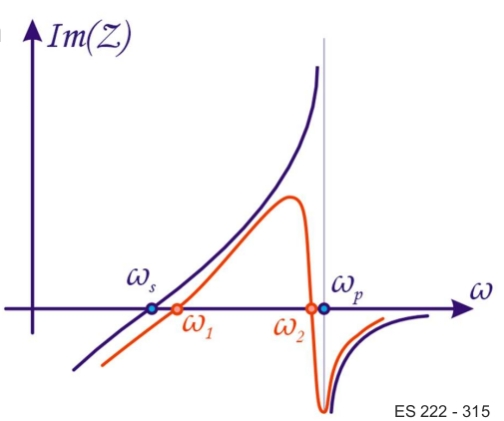
\includegraphics[width=6cm]{figures/ch11/quartz2.jpg}
	\captionof{figure}{}
	\label{fig:quartz2}
\end{minipage}%
\begin{minipage}{.5\textwidth}
	\centering
	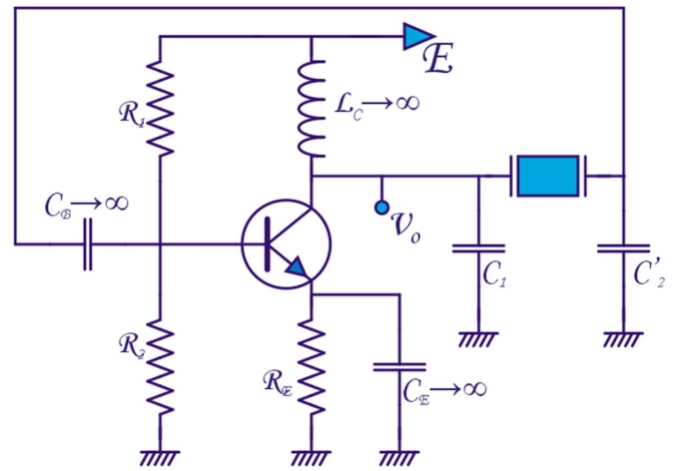
\includegraphics[width=7cm]{figures/ch11/quartz3.jpg}
	\captionof{figure}{}
	\label{fig:quartz3}
\end{minipage}

We can construct a Colpitts oscillator with a quartz crystal instead of an inductor $L$, as in figure \ref{fig:quartz3}. This oscillator has an oscillation frequency $\omega_0 = \frac{1}{LC}$ with $C$ the parallel combination of $C_1$ and $C_2$. This frequency necessarily lies between $\omega_s$ and $\omega_p$ because $Z$ is only inductive in this region, and the corresponding inductance is determined by the red curve in figure \ref{fig:quartz2}. If $\omega_0$ lies outside this region, $Z$ would be capacitive and the oscillator would not work. If the frequency $\omega_0$ would try to drift, e.g. because of a variation in $C$, the inductance $L$ would also change, and the positive slope of $Z$ will adjust $L$ so that $\omega_0$ remains relatively constant: 
$$C \uparrow  \; \Rightarrow \omega_0 = \sqrt{\frac{1}{LC}} \downarrow \; \Rightarrow L = Z(j\omega_0) \downarrow  \; \Rightarrow \omega_0 \uparrow$$
This means the system is self-corrective and it is also why the quartz oscillator is very stable.

\section{Relaxation Oscillator}
\label{sec:relaxation}
The oscillators we saw so far were all based on the principle that for a certain frequency $\omega_0$, we want to create a loop gain $T(j\omega_0) = 1$. Another type of oscillator is the \emph{relaxation oscillator}, which is based on the instability of an amplifier. We configure the circuit such that the output of an amplifier keeps switching between high and low, and a capacitor elsewhere in the circuit will eternally be charged and discharged (the \emph{relaxation} of a capacitor). The output waveform will no longer be a sinusoid, but a block or triangle signal.\\
Whether a circuit is stable or not can be verified by Lyapounov's theorem. To do this:
\begin{itemize}
	\item First find all the fixed points of the circuit, i.e. the solutions of the governing equations with all time derivatives and inputs set to zero.
	\item Linearize the system around these solutions.
	\item Identify how the operating point moves as time $t$ increases (typically, the solutions have an exponential behavior). % or when small perturbations are applied 
	\item If the operating point returns to the solution, the system is stable. If not, the system might be unstable.
\end{itemize} 
As an example, consider the circuit in figure \ref{fig:relaxation1}, with its operating equations:
\begin{align*}
	v_o &= \phi(v) \text{ (the OPAMP characteristic)}\\
	i &= \frac{v_i + v}{R} = C \; \frac{dv_c}{dt} \\
	v_o &= -v + v_c
\end{align*}
If $\frac{dv_c}{dt} = 0$, we find the fixed point - with the input set to $0$: $i = 0, v_i = 0, v = 0, v_o = 0$.

\begin{minipage}{.5\textwidth}
	\centering
	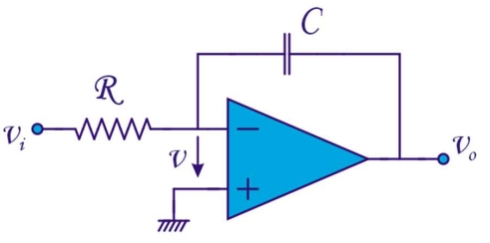
\includegraphics[width=7cm]{figures/ch11/relaxation1.jpg}
	\captionof{figure}{An integrator}
	\label{fig:relaxation1}
\end{minipage}%
\begin{minipage}{.5\textwidth}
	\centering
	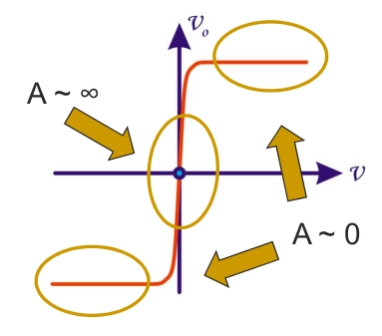
\includegraphics[width=5cm]{figures/ch11/relaxation2.jpg}
	\captionof{figure}{OPAMP function: $v_o = \phi(v)$}
	\label{fig:relaxation2}
\end{minipage}
\\

We linearize the operating equations around this fixed point. To do this, we approximate $v_o = \phi(v)$ by three different linear regions as in figure \ref{fig:relaxation2}: two with gain $A \approx 0$, and one with $A \approx \infty$. The fixed point $v = v_o = 0$ is associated with $A \approx \infty$.

\begin{align*}
	v_o &= A\;v = -v + v_c \Rightarrow v = \frac{v_c}{A+1}\\
	(A+1) v_i  &= (A + 1) RC \; \frac{dv_c}{dt} - v_c \\
	\Rightarrow v_c(t) &= (1 + A) v_i (e^{t/(1 + A)RC} - 1)
\end{align*}
So this system is unstable because $v_c \rightarrow \infty$ if $t \rightarrow \infty$ (except when $v_i = 0$). This is evident from the exponent in $e^{\alpha t}$: if $\alpha > 0$, the behavior is unstable, as we find here for $\alpha = \frac{1}{(1 + A)T}$. The origin of the exponential behavior is a first-order differential equation:
$$
\frac{dv_c}{dt} = \alpha \; v_c + v_i
$$
which is stable if $\alpha < 0$.\\
Because $e^x \approx 1 + x$ when  $x$ is small, we find that for small values of $t$, $v_c(t) \approx \frac{t}{RC} v_i$, i.e. we find the expression for an integrator, as expected.\\

Let's apply this to the circuit in figure \ref{fig:relaxation3}, which is a \emph{relaxation oscillator}.
\begin{figure}[h!]
	\centering
	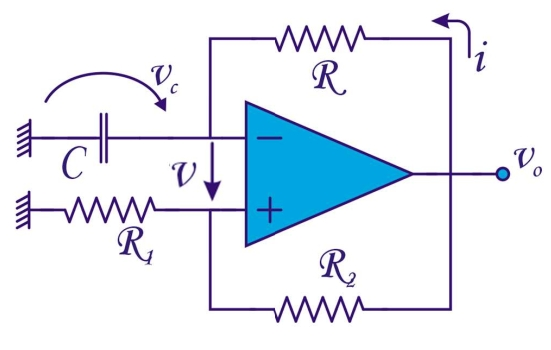
\includegraphics[width=8cm]{figures/ch11/relaxation3.jpg}
	\caption{A relaxation oscillator}
	\label{fig:relaxation3}
\end{figure}

The operating equations are:
\begin{align*}
	v_o &= \phi(v) \\ %\approx A\; v\\
	i   &= C\;\frac{dv_c}{dt} \\
	v_o - v_c &= R\;i \\
	v + v_c &= \frac{R_1}{R_1 + R_2} v_o = k\; v_o
\end{align*}
These equations have a fixed point around $v_o = v_c = v = 0$ and $i=0$. When we linearize around this point (i.e. we set $v_o = A\; v$), we find:
\begin{align*}
	v_c = v_o - R\;i = A v - RC\;\frac{dv_c}{dt}\\
	v  + v_c = k v_o = Ak\; v \\
	\rightarrow v_c = (Ak - 1) \; v \\
	\rightarrow v_c = \frac{A}{Ak - 1} v_c - RC\; \frac{dv_c}{dt}
\end{align*}
and so:
\begin{align*}
	v_c &= \frac{Ak-1}{Ak-A-1} RC \frac{dv_c}{dt} \\
		&= \frac{k - 1/A}{1 - k + 1/A} RC \frac{dv_c}{dt}
\end{align*}
The stability criterion is thus:
$$
\frac{k - 1/A}{1 - k + 1/A} > 0
$$
or in other words: $A > \frac{1}{k}$.\\
To understand how the circuit works, assume that $v_o = E$. Then capacitor $C$ is charging and the voltage at the negative input increases. At some point in time, the voltage at $v^-$ becomes larger than $v^+ = \frac{R_1}{R_1 + R_2} E$ and because of the large gain, the output voltage switches to $v_o = -E$. The capacitor $C$ has still a charge of $C \frac{R_1}{R_1 + R_2} E $ on it, so $v^-$ changes abruptly to $ -E + \frac{R_1}{R_1 + R_2} E$. Now, the process reverses: the capacitor starts to discharge, the voltage at $v^-$ decreases and suddenly $v$ becomes positive and the output switches again. The process is shown in figure \ref{fig:relaxation4}.\\
\begin{figure}[h!]
	\centering
	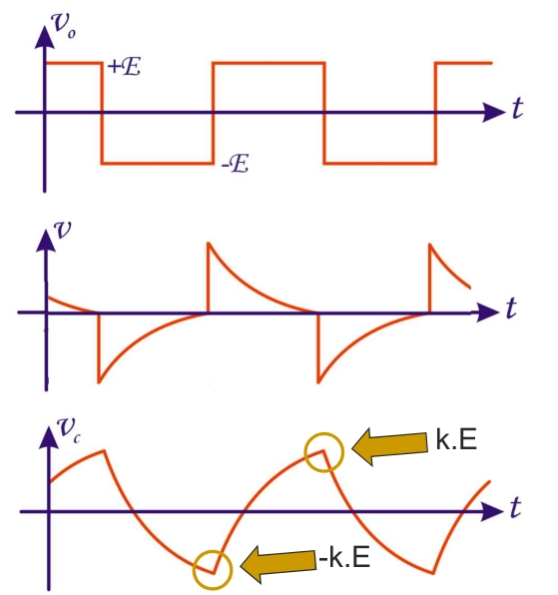
\includegraphics[width=6cm]{figures/ch11/relaxation4.jpg}
	\caption{}
	\label{fig:relaxation4}
\end{figure}
When $C$ is charging or discharging, we can write:
$$
v_c(t) = v_c(\infty) + (v_c(0) - v_c(\infty)) e^{-t/T} 
$$
With this equation, we can compute the frequency of oscillation: the switching criterion is when $v=0$, i.e. at time $t=T$ when 
$$ kE = E + (-kE - E) \; e^{-\frac{T}{2RC}} $$
and thus $T = 2RC \ln \frac{1+k}{1-k}$.

\section{The Fantastron}
\label{ch:fantastron}

The \emph{fantastron} (figure \ref{fig:fantastron1}) is a type of relaxation oscillator that consists of
\begin{enumerate}
	\item An unstable comparator (also called a \emph{Schmidt trigger}, see also section \ref{sec:schmidt}): if $v_p$ switches sign, the output voltage will switch from $+E$ to $-E$ because the feedback happens on $v^+$.
	\item An integrator with time constant $RC$.
\end{enumerate}

\begin{figure}[h!]
	\centering
	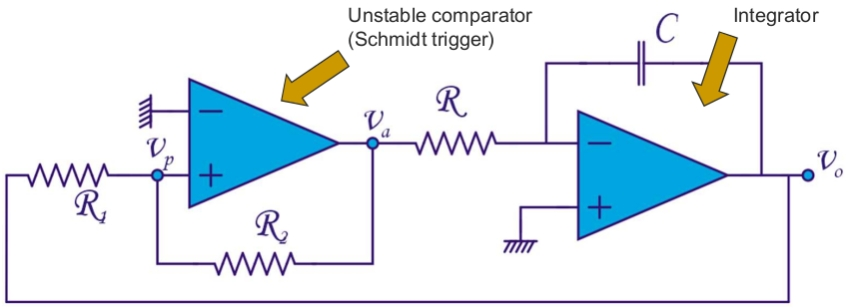
\includegraphics[width=12cm]{figures/ch11/fantastron1.jpg}
	\caption{The Fantastron}
	\label{fig:fantastron1}
\end{figure}

With $v_a$ equal to $\pm E$, we can write the voltage $v_p$ as (Millman):
$$
v_p = \frac{R_2 v_o \pm R_1 E}{R_1 + R_2}
$$
If $v_p > 0$, $v_a = E$, and the integrator will start to integrate down with slope $-\frac{E}{RC}$, until the output reaches $v_o = \pm E \frac{R_1}{R_2}$. At that time, $v_p$ will become negative, $v_a$ switches suddenly to $v_a = -E$, and the process starts all over again in the other direction. The waveforms for $v_a$ and $v_o$ are shown in figure \ref{fig:fantastron2}. In this circuit, we have simultaneously access to a block signal as to a triangle waveform.

\begin{figure}[h!]
	\centering
	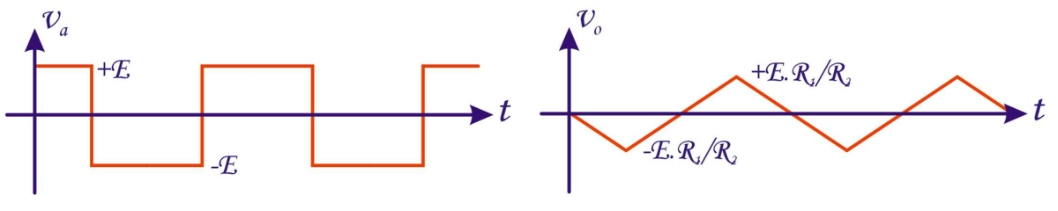
\includegraphics[width=14cm]{figures/ch11/fantastron2.jpg}
	\caption{}
	\label{fig:fantastron2}
\end{figure}
The period is thus determined by when $v_p$ switches sign. One half period $\frac{T}{2}$ corresponds to the time for $v_o$ to go from $-\frac{R_1}{R_2}E$ to $+\frac{R_1}{R_2}E$ with slope $\frac{E}{RC}$:
$$
- \frac{R_1}{R_2}E + \frac{E}{RC} \frac{T}{2} = \frac{R_1}{R_2} E
$$
and so:
$$
T = 4 \; \frac{R_1}{R_2}\;  RC
$$